\chapter{Etude avec utilisation du test Tomatis en clinique psychiatrique.}
Nous savons que la musicothérapie est de plus en plus intégrée dans
les milieux psychiatriques. Nous avons choisi ce terrain d'étude car 
nous  travaillons dans ce domaine  à temps partiel comme musicothérapeute.
\section{Cadre de travail}
 La Privatklinik
de Meiringen est  spécialisée en
addictologie dans le canton de Berne. Elle dispose d'une capacité de 195 lits, 33 médecins et
psychologues, secondés par 177 soignants qui assurent le suivi du
patient. Regula Lehman, musicothérapeute à temps complet, et nous-même avons
collaboré  pour l'organisation de la mise en place de l'étude. Celle-ci porte sur un même type de
population dans le contexte et cadre  précis d'une prise en charge globale
par les médecins, les psychologues, les thérapeutes: physio--,
ergo--, art--,musico--,corporel etc. et les divers ateliers de créativité proposés dans
cette clinique. 

Pathologies:  burnout, dépendances,
dépression.
Moyenne d'âge:  entre 20 à 60 ans, masculin et
féminin quasi égale. 
En raison des problèmes de surdité souvent observée à partir de 60 ans, nous avons omis volontairement les patients au-delà de cet âge.
\section{Organisation d'étude}

Au préalable, nous avons fait circuler une
feuille d'information pour expliquer notre démarche d'évaluation sur
l'hypothèse de la transformation de l'écoute du patient lors de son
séjour en thérapie. \emph{Information für Mitwirkende an der klinischen
Studie\  "Evaluierung des aktiven Hörvermögens" }. 
 
 \section{Contact avec les patients}
 
 Nous avons
préparé les patients avec une explication préalable. Ensuite,
ceux-ci ont signé officiellement à chaque fois leur
accord pour cette participation  \emph{"Eine schriftliche Einbewilligung zum
Test"} avant de passer ces tests dont nous nous sommes occupées.
  \footnote{Regula
  Lehmann, musicothérapeute  à 90\%  à la clinique de Meiringen} Deux groupes, un témoin, sans
musicothérapie et un autre avec ont été organisés, avec un séjour moyen 4 semaines de thérapies dans cet établissement et un facteur non négligeable d'entrées et des sorties très aléatoires.


\begin{itemize}
	\item 10 patients testés, groupe A en musicothérapie : un
          premier test avant leur prise en charge en musicothérapie;
          puis un deuxième test \textdegree{} : après 4 semaines de
          clinique.
	\item 10 patients testés, groupe B de contrôle qui est un groupe sans musicothérapie,
	toujours dans le même contexte, c.à.dire la clinique, le suivi et les mêmes protocoles que l'autre groupe. Un premier test avant
	le début des autres thérapies puis un deuxième test, après 4 semaines. 
	Les tests ont été faits en avril, mai, juin, juillet, septembre et octobre 2017.
	Nous avons réalisé en tout 40 tests d'écoute Tomatis. 
	Précision importante : Pour cette étude, nous avons intentionnellement exclu la thérapie avec les musiques traitées et appliquées avec Tomatis, en nous restreignant  à ce lieu où l'application de cette forme de thérapie n'existe pas.
	Durée des tests : Chaque test Tomatis a une durée  moyenne de 50 à 60  minutes par patient. Pour chacun, nous avons donc réalisé en tout deux heures de tests d'écoute avec un entretien, et leur avons demandé en plus de remplir le questionnaire WHOQOL (20mn).
\end{itemize}

\section{Le WHOQO-Bref}

Nous avons utilisé et fait en parallèle le test WHOQO-Bref avant et
après pour avoir une variable supplémentaire pour confirmer en
parallèle supposée de l'action de la musicothérapie sur une éventuelle modification de l'écoute.  C'est une
version test de 1997 issue du Programme sur la santé mentale,
Organisation mondiale de la santé, Genève. Il y a 26 questions, que le
patient a rempli lui-même en présence du thérapeute, avant le test
d'écoute. La durée pour les remplir a varié de 8 à 10 minutes en
moyenne.  Il a eu 26 tests WHOQO-Bref.
Il y a quatre domaines testés : physique, psychologique, relations sociales et environnement.
\begin{enumerate}
	\item  Le domaine de la perception physique comprend l' activité quotidienne// la dépendance et/ou l'assistance médicale// la fatigabilité, l'énergie//la mobilité// la douleur// le sommeil// la capacité de travail//
	
		 \item Le domaine psychologique :  image de soi, apparence// ressentis positifs et négatifs// estime de soi// spiritualité, croyances personnelles, religion// mémoire et concentration, apprentissage, pensée.
		
			\item Le domaine des relations sociales : relations personnelles// soutien social// vie sexuelle.
			
			\item Le domaine de l'environnement : l'environnement domestique et  physique (pollution, bruit, trafic, climat)// la situation financière//  la liberté, la sécurité physique et morale// l'accessibilité et qualité de la santé// les opportunités de détente, loisirs et d'acquisition d'informations// le transport// 
		\end{enumerate}
		
	


 \section{Les tests d'écoute} 	
 
 \paragraph{Le test d'écoute Tomatis est une traduction graphique de l'écoute, elle permet d'objectiver la qualité de l'écoute.} 
 
  \begin{enumerate}
 	\item les seuils d'écoute
 	\item le son : dB, 
 	\item le volume de $-20$ à 90 % finesse typo: le signe moins des mathématiques.
 	\item les fréquence, de 125 à 8000.   \label{chapitre 6.2t} % mets une étiquette plus
 	% ``parlante'' stp, genre ``parametres_test_ecoute''.
 	\item la courbe, par l'observation des courbes d'écoute relevées
 	en comparaison avec la courbe dite idéale : équilibre,
 	déséquilibre, harmonie, disharmonie.  
 	\item équilibre, déséquilibre graphique entre les deux oreilles et entre les deux courbes mesurées par oreille: observation des croisements, des parallèles, des
 	écarts importants entre les courbes aériennes et osseuses\footnote{Remarque :
 		Un carré sur le graphique représente une différence de 5dB en
 		volume.}.
 	\item une modification perçue ou non comme évolutive lors des transformations graphiques de courbes
 	\item  Informations croisées avec les informations récoltées   par les 3 zones du test d'écoute: ........
 	\item une constatation de la posture d'écoute et de la qualité de
 	la voix. La voix se caractérise par son volume, son timbre, sa mélodie et son langage. 
 	
 	
 Nous pouvons faire ainsi le descriptif général de la voix d'un patient dépressif :
 	\begin{enumerate}
 		\item le volume : basse intensité
 		\item la mélodie : monotone, sans modulation
 		\item le timbre : mauvaise qualité due à une pertes des harmoniques
 		\item le langage : difficulté d'élocution
 	\end{enumerate}
 	
 		
 	
 	
 	
 	\section{Les graphiques}
 	
 	\lipsum[1]
 	
 	\subsection{Situation au début}
 	
 	\lipsum[1]
 	
 	\begin{figure}[tbh]
 		\centering
 		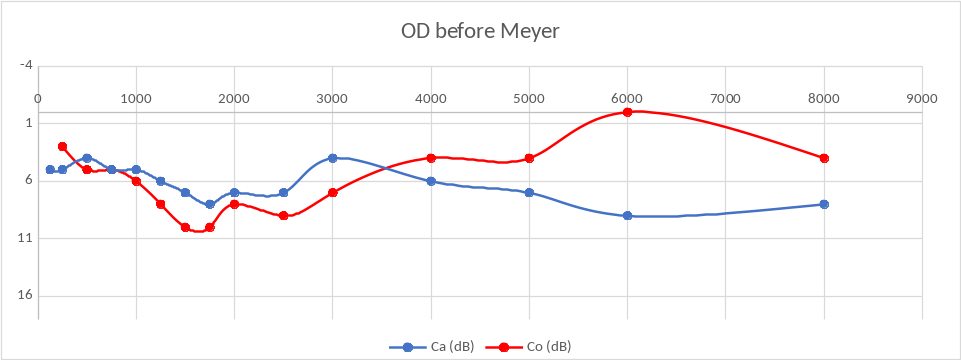
\includegraphics[width=0.7\linewidth]{images/clinique/od_before_meyer.png}
 		\caption{OD Avant Meyer}
 		\label{fig:odbeforemeyer}
 	\end{figure}
 	
 	\lipsum[1]
 	
 	
 	
 	
 	\begin{figure}
 		\centering
 		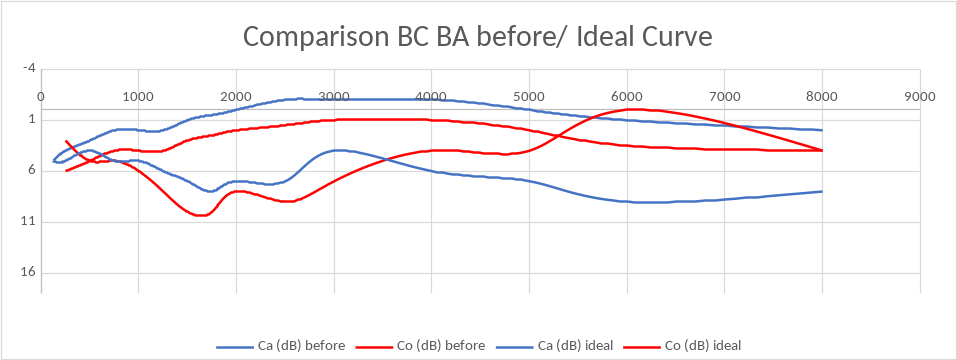
\includegraphics[width=0.7\linewidth]{images/clinique/comparison_bc_ba_before_vs_ideal_curve_meyer.png}
 		\caption[Avant vs courbe idéale]{Comparaison avant vs courbe idéale}
 		\label{fig:comparisonbcbabeforevsidealcurvemeyer}
 	\end{figure}
 	
 	
 	\subsection{Situation après}
 	\lipsum[1]
 	\begin{figure}[h]
 		\centering
 		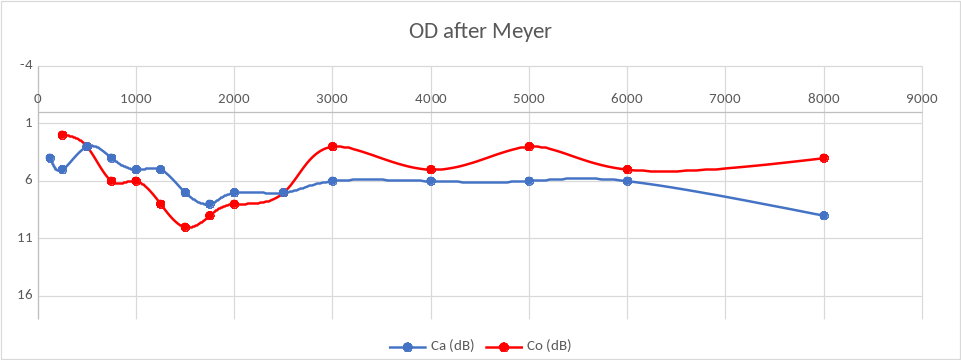
\includegraphics[width=0.7\linewidth]{images/clinique/od_after_meyer.png}
 		\caption{OD après vs courbe idéale}
 		\label{fig:odaftermeyer}
 	\end{figure}
 
 \lipsum[1]
 
 \begin{figure}[bh]
 	\centering
 	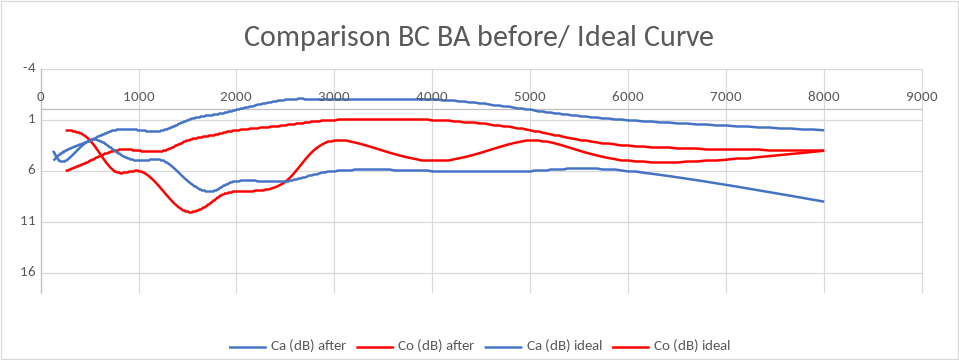
\includegraphics[width=0.7\linewidth]{images/clinique/comparison_bc_ba_after_vs_ideal_curve_meyer.png}
 	\caption{Comparaison après}
 	\label{fig:comparisonbcbaaftervsidealcurvemeyer}
 \end{figure}
 
 	
 	
 	\section{Les résultats}
 	
 	....
 	
 	
 	
 \section{Les résultats et réflexions}	
Le manque de temps a été le principal facteur  réducteur
de tests valables, les départs imprévus des patients, et/ou leur
absence momentanée ( visite du psychologue, maladie, etc.). rajoutés au peu de temps de travail( 10\% )ainsi qu'à la
contingence difficile due à la distance séparant Genève du lieu de travail ( Meiringen)
: comment planifier un départ imprévu d'un patient !? il a fallu parfois
faire trois heures de route pour effectuer les tests finaux d'un ou deux
patients.
  
Par conséquent,  de nombreux tests sont restés 
incomplets et n'ont pu
être validés car ils ne remplissaient pas toutes les conditions requises.  En définitive, sur 40 tests d'écoute Tomatis et 26 tests
WHOQO-Bref, nous avons choisi de ressortir l'étude pour le groupe A de
5 patients effectifs en musicothérapie, tests complets, et le groupe
témoin B de 5 patients sur 9 effectifs, sans musicothérapie et tests
complets. 
 

  
\paragraph{Les résultats}
  
  De manière très générale, les résultats obtenus ne
  sont pas significatifs.  La prise en charge en musicothérapie a eu lieu
  une fois par semaine pendant une heure, ce qui semble trop court pour observer un changement important. Nous pourrions émettre la supposition suivante :  est-ce qu'un un travail journalier, régulier aurait été indiqué pour des résultats plus rapidement visibles avec le test?
  Est-ce qu'une immersion plus intensive en musicothérapie transformerait l'écoute des patients ? 
   En comparaison avec des
  modifications importantes de courbes des tests observées généralement  lors d' une écoute
  régulière de deux heures par jour de musique pendant 15 jours, --en référence à l'entrainement des muscles de l'oreille chez Tomatis, qui, nous le rappelons, est une pédagogie de l'écoute--, il aurait été intéressant de pouvoir faire cette étude comparative dans cette clinique. Ainsi, nous aurions pu éventuellement mettre en avant  l'absolue nécessité de créer et d'instaurer systématiquement la musicothérapie dans de nombreuses institutions mais aussi  de la développer beaucoup plus intensément  si elle est déjà existante.
  Nous sommes clairement en présence d'une ébauche d'études, avec des pistes
  suggérées. 
  Cette étude est un mixe: quantitatif et qualitatif. Nous avons ainsi pris l'option de nous tenir à une
  observation, celle de la transformation de l'écoute.
  
  A fortiori, relevons le cas fort intéressant  d'une patiente du groupe B( sans
  musicothérapie) : lors du test, surprise d'apprendre en voyant son écoute que la musique pouvait la modifier, elle s'est mise à écouter assidûment du Mozart pendant son séjour en clinique, entre le 1° test et le second test.  Les résultats
  graphiques obtenus lors de sa sortie sont clairement significatifs
  et de plus sont en concordance avec le WHOQ-Bref!  
  Par cnséquent, le test d'écoute a permis de lui faire prendre conscience d'une part que son écoute lui appartenait personnellement et d'autre part, qu'elle pouvait elle-même avoir un impact et jouer un rôle non seulement sur son écoute mais aussi sur sa propre  transformation.



   
   
   
   
  \end{enumerate}










